% vim: spelllang=en:
\documentclass[12pt]{letter}
\usepackage[a4paper,vmargin={1.3in,1.3in},foot=0.71in]{geometry}

% input common settings
% vim: nospell
% LOAD PACKAGES #############################################################
% to select features depending on engine
\usepackage{ifpdf,ifluatex}

% allow use of . in filenames
\usepackage{grffile}

% spacing
\usepackage{indentfirst,xspace}

% basic graphics packages
\usepackage{graphicx,xcolor}

% tables
\usepackage{booktabs}
\renewcommand{\arraystretch}{1.2}  % more space between rows

% remove extra space at borders of table (lines are then justified with text)
\let\oldtabular\tabular
\let\endoldtabular\endtabular
\renewenvironment{tabular}[1]{\begin{oldtabular}{@{}#1@{}}}{\end{oldtabular}}

% basic mathematics packages
\usepackage{amsmath,amssymb}

% fonts
\ifluatex
  \usepackage{fontspec}
  \defaultfontfeatures{Ligatures=TeX}
  % Font shapes:
  % UprightFont, BoldFont,
  % ItalicFont, BoldItalicFont,
  % SlantedFont, BoldSlantedFont,
  % SmallCapsFont
  \setmainfont{LinLibertine_}[
    Extension = .otf,
    UprightFont = *R,
    BoldFont = *RB,
    ItalicFont = *RI,
    BoldItalicFont = *RBI,
    Numbers = {Proportional,OldStyle},
    SmallCapsFeatures = { LetterSpace=5, Kerning=On },
  ]
  \setsansfont{LinBiolinum_}[
    Extension = .otf,
    UprightFont = *R,
    BoldFont = *RB,
    ItalicFont = *RI,
    BoldItalicFont = *RBO,
    Numbers = {Proportional,OldStyle},
    SmallCapsFeatures = { LetterSpace=7, Kerning=On },
  ]
  \setmonofont{iosevkatermslab}[
    UprightFont = *nerdfontcomplete,
    BoldFont = *boldnerdfontcomplete,
    ItalicFont = *italicnerdfontcomplete,
    BoldItalicFont = *bolditalicnerdfontcomplete,
    SlantedFont = *obliquenerdfontcomplete,
    BoldSlantedFont = *boldobliquenerdfontcomplete,
    Scale=MatchLowercase,
  ]
  \usepackage{unicode-math}
  \setmathfont{Asana-Math.otf}

  % lining figures
  \newcommand\lfstyle{\addfontfeature{Numbers=Lining}}
  \newcommand\textlf[1]{{\lfstyle #1}}
\else
  \usepackage[T1]{fontenc}
  \usepackage[utf8]{inputenc}
  \usepackage[p,osf]{newtxtext}  % old-style figures in text mode
  \usepackage{newtxmath}
\fi
\newcommand\Arabic[1]{\textlf{\arabic{#1}}}  % Arabic uses lining figures

% more mathematics packages
\usepackage{siunitx,commath,xfrac}

% ASYMPTOTE PREAMBLE ########################################################
\ifluatex
  \ifx\pdfpagewidth\undefined\let\pdfpagewidth\paperwidth\fi
  \ifx\pdfpageheight\undefined\let\pdfpageheight\paperheight\fi
\else
  \let\paperwidthsave\paperwidth\let\paperwidth\undefined
  \let\paperwidth\paperwidthsave
\fi
\newbox\ASYbox
\newdimen\ASYdimen
\def\ASYprefix{}
\long\def\ASYbase#1#2{\leavevmode\setbox\ASYbox=\hbox{#1}%\ASYdimen=\ht\ASYbox%
\setbox\ASYbox=\hbox{#2}\lower\ASYdimen\box\ASYbox}
\long\def\ASYaligned(#1,#2)(#3,#4)#5#6#7{\leavevmode%
\setbox\ASYbox=\hbox{#7}%
\setbox\ASYbox\hbox{\ASYdimen=\ht\ASYbox%
\advance\ASYdimen by\dp\ASYbox\kern#3\wd\ASYbox\raise#4\ASYdimen\box\ASYbox}%
\setbox\ASYbox=\hbox{#5\wd\ASYbox 0pt\dp\ASYbox 0pt\ht\ASYbox 0pt\box\ASYbox#6}%
\hbox to 0pt{\kern#1pt\raise#2pt\box\ASYbox\hss}}%
\ifpdf
  \long\def\ASYalignT(#1,#2)(#3,#4)#5#6{%
  \ASYaligned(#1,#2)(#3,#4){%
  \special{pdf:q #5 0 0 cm}%
  }{%
  \special{pdf:Q}%
  }{#6}}
  \long\def\ASYalign(#1,#2)(#3,#4)#5{\ASYaligned(#1,#2)(#3,#4){}{}{#5}}
  \def\ASYraw#1{#1}
\else
  \long\def\ASYalignT(#1,#2)(#3,#4)#5#6{%
  \ASYaligned(#1,#2)(#3,#4){%
  \special{ps:gsave currentpoint currentpoint translate [#5 0 0] concat neg exch neg exch translate}%
  }{%
  \special{ps:currentpoint grestore moveto}%
  }{#6}}
  \long\def\ASYalign(#1,#2)(#3,#4)#5{\ASYaligned(#1,#2)(#3,#4){}{}{#5}}
  \def\ASYraw#1{
  currentpoint currentpoint translate matrix currentmatrix
  100 12 div -100 12 div scale
  #1
  setmatrix neg exch neg exch translate}
\fi


\setlength{\parskip}{3em} % paragraph spacing
\pagenumbering{gobble}    % page numbering (gobble removes it)

% background image
\usepackage[scale=1,angle=0,opacity=1]{background}
\backgroundsetup{contents={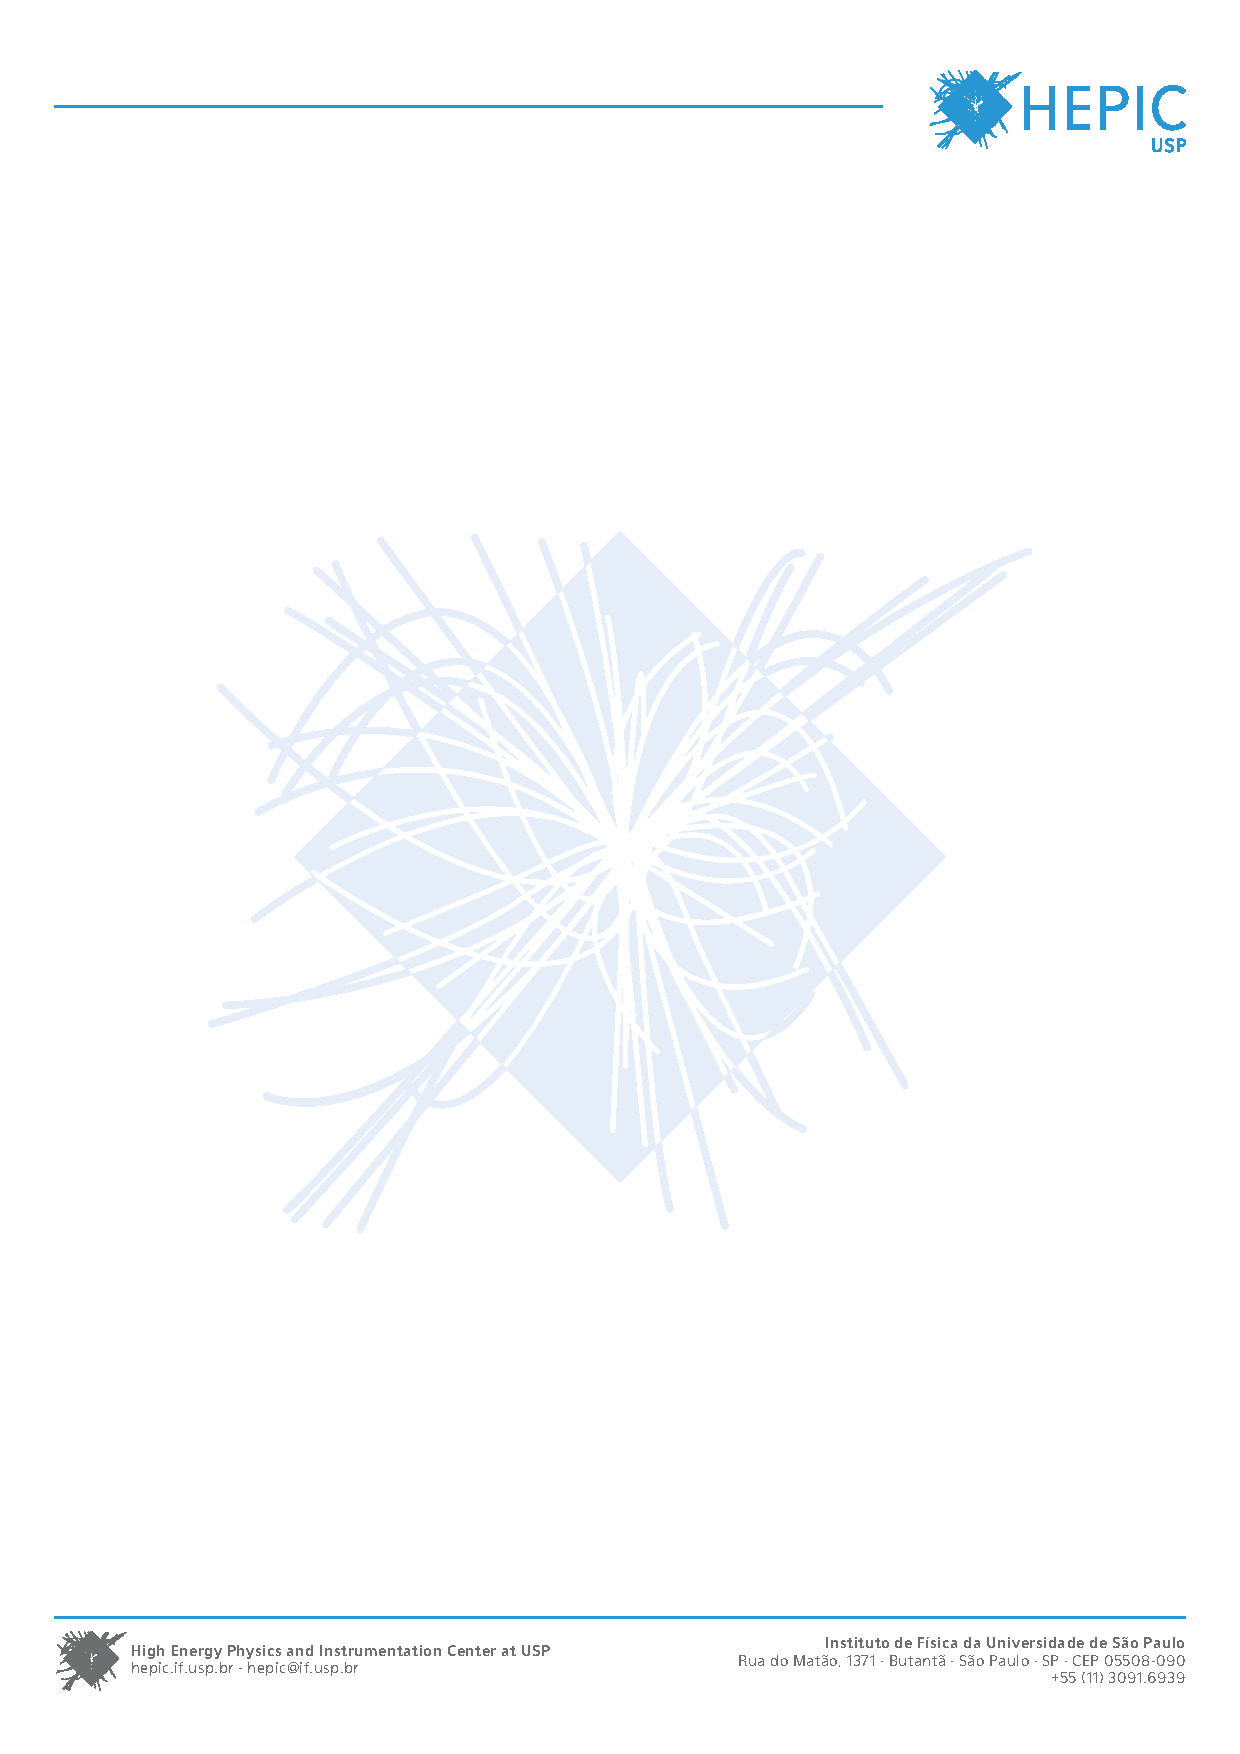
\includegraphics[width=\paperwidth]{letterhead}}}
% default text color: HEPIC=6D6E70
\usepackage{xcolor}\makeatletter\AtBeginDocument{\color[HTML]{6D6E70}\global\let\default@color\current@color}\makeatother

% common data
\title{Declaration}
\date{\today}
\name{Caio Alves Garcia Prado}
\address{São Paulo}

\begin{document}
\begin{letter}{}
\makeatletter\begin{center}\Large\textbf{\@title}\end{center}\makeatother\vspace\parskip

  \makeatletter
\newcommand\getsize[1]{{#1\global\let\@value\f@size}\@value}
\newcommand\getskip[1]{{#1\global\let\@value\f@baselineskip}\@value}
\newcommand\printsize[1]{{\ttfamily\string#1} & \getsize{#1} & \getskip{#1}}
\makeatother

% Draw a line showing a font metric
%  #1 color, #2 vertical position, #3 label
\newcommand{\drawmetric}[3]{%
  \clap{%
    \color{#1}\rule[#2]{9.8cm}{0.05pt}%
    \raisebox{#2}{\scalebox{0.3}{\tiny\selectfont\sffamily #3}}%
  }%
}
\newcommand\drawallmetrics{%
  \drawmetric{red}{0pt}{baseline}%
  \drawmetric{blue}{1ex}{x-height}%
  \drawmetric{red}{\fontcharht\font`X}{cap-height}%
  \drawmetric{cyan}{\the\fontdimen22\textfont2}{math axis}%
}

\newcommand\tenglish{%
    normal, \textbf{bold,} \textit{italic,} \textsl{slanted,} %
    \textbf{\textit{bolditalic,} \textsl{boldslanted,}} %
    0123456789%
}
\newcommand\tchinese{%
    普通,\textbf{粗体,}\textit{斜体,}\textsl{倾斜,}%
    \textbf{\textit{粗斜体} \textsl{粗倾斜体,}}%
    0123456789%
}
\newcommand\test{\noindent\tenglish\\\textsc{\tenglish}\\\tchinese\vspace*{1em}}

\newcommand\fontsample[1][1]{\begin{center}\scalebox{#1}{
\begin{minipage}{13.4cm}
\begin{center}
    \sisetup{
        table-format = 3.2,
        table-alignment = center,
    }
    \begin{tabular}{
            lSS[table-space-text-post=~pt]
            lSS[table-space-text-post=~pt]}
        \toprule
        {\textbf{Size}} & {\textbf{Value}} & {\textbf{Skip}}
            & {\textbf{Size}} & {\textbf{Value}} & {\textbf{Skip}} \\

        \midrule
        \printsize\tiny         & \printsize\large \\
        \printsize\scriptsize   & \printsize\Large \\
        \printsize\footnotesize & \printsize\LARGE \\
        \printsize\small        & \printsize\huge  \\
        \printsize\normalsize   & \printsize\Huge  \\
        \bottomrule
    \end{tabular}
    \vspace*{1em}

    \noindent\clap{\textrm{abcde} \textsf{abcde} \texttt{abcde}}\drawallmetrics{}

    \noindent\clap{
    \textrm{\lfstyle01234ABCDE}
    \textsf{\lfstyle01234ABCDE}
    \texttt{\lfstyle01234ABCDE}
    \textrm{中国普通话}
    }\drawallmetrics{}

    \noindent\clap{
    \textrm{中国普通话}
    \textrm{\textit{中国普通话}}
    \textsf{中国普通话}
    \textsf{\textit{中国普通话}}
    \texttt{中国普通话}
    }\drawallmetrics{}
\end{center}
\vspace*{1em}

\textrm{\test}\\ \textsf{\test}\\ \texttt{\test}
\end{minipage}}\end{center}}


\makeatletter
  \par\nobreak\vspace{\parskip}\stopbreaks\noindent\raggedleft
  \fromaddress, \@date\\
  \vspace{2\parskip}
  \newlength\underlinelength
  \settowidth\underlinelength\fromname
  \addtolength\underlinelength{2ex}
  \rule\underlinelength\linethickness\\
  \fromname\hspace*{1ex}
\makeatother
\end{letter}
\end{document}
